\documentclass[12pt, a4paper, reqno, oneside]{book}
\usepackage{amsmath,amsxtra,amssymb,latexsym, amscd,amsthm}
\usepackage{indentfirst}
\usepackage{color}
\usepackage[utf8]{vietnam}
\usepackage{amsmath}
\usepackage[mathscr]{eucal}
\usepackage{amsfonts}
\usepackage{graphicx}
\usepackage{cases}
\usepackage{listings}
\usepackage{multicol}
%\input setbmp
\usepackage[unicode]{hyperref}
\usepackage{titledot}
\titlename{Chương}
%+ Can le van ban
\setlength{\oddsidemargin}{0in}
\setlength{\textwidth}{6.in}
\setlength{\topmargin}{-0.5in}
\setlength{\textheight}{9.25in}
\renewcommand{\baselinestretch}{1.5}

\evensidemargin 5.4mm
\oddsidemargin 5.4mm
%+ Dinh nghia mot so ky hieu toan hoc.
\def\B{\mathscr B}
\def\one{\mathbf 1}
\def\R{{\mathbb R}}
\def\LL{{\mathbb L}}
\newcommand\abs[1]{|#1|}
\newcommand\set[1]{\{#1\}}
\newcommand\norm[1]{||#1||}
\DeclareMathOperator{\vrai}{vrai}
\DeclareMathOperator{\const}{const}
\newcommand{\eoproof}{\hfill $\square$}
\newcommand{\spro}[1]{\left<#1\right>}
\newcommand{\argmin}{\arg\min}

\renewcommand{\theequation}{\arabic{chapter}.\arabic{section}.\arabic{equation}}
\newtheorem{lemma}{\bf Bổ đề}[section]
\newtheorem{theorem}{\bf Định lý}[section]
\newtheorem{proposition}{\bf Mệnh đề}[section]
\newtheorem{corollary}{\bf Hệ quả}[section]
\newtheorem{definition}{\bf Định nghĩa}[section]
\newtheorem{remark}{\bf Chú ý}[section]

\definecolor{mygreen}{RGB}{28,172,0} % color values Red, Green, Blue
\definecolor{mylilas}{RGB}{170,55,241}






%+ Bat dau tai lieu tai day.
\begin{document}
%+ ====================================================





\makeatletter
\renewcommand{\ps@myheadings}{
\renewcommand{\@oddhead}{\textsf{Các mô hình ngẫu nhiên và ứng dụng}\hfil\textrm{\thepage}}
\renewcommand{\@oddfoot}{\textsf{KSTN Toán Tin K61 - Viện Toán ứng dụng và Tin học}\hfil}
}
\makeatother 

%+ Page style
\newpage
\input bia

\tableofcontents

\newpage
\input loimodau

\newpage
\setcounter{chapter}{0}
\chapter{Giới thiệu bài toán}
Với sự tiến bộ nhanh chóng trong công nghệ thương mại điện tử, việc sử dụng thẻ tín dụng để phục vụ nhu cầu trong đời sống cũng như trong doanh nghiệp đã tăng lên một cách đáng kể. Ngày nay, thẻ tín dụng đang trở thành phương thức thanh toán phổ viến nhất trong việc mua hàng trực tuyến, cũng như mua hàng trực tiếp, bởi vậy mà các trường hợp gian lận thẻ tín dụng cũng đang gia tăng. Trong bài báo cáo này, nhóm chúng em sử dụng mô hình Makov ẩn (Hiden Makov Model – HMM) để nghiên cứu, mô hình hóa chuỗi hoạt động trong việc xử lý thông tin giao dịch thẻ tín dụng và chỉ ra cách phát hiện gian lận.
\section{Thẻ tín dụng}
Chiếc thẻ ngân hàng đầu tiên được xuất hiện từ năm 1946 với cái tên "Chard-lt", do John Biggins ở Brooklyn nghĩ ra. Khi khách hàng mua sắm, hóa đơn được chuyển đến ngân hàng của Biggins. Ngân hàng trả tiền cho người bán và sau đó khách hàng trả tiền cho ngân hàng. Điểm trừ là loại thẻ nay chỉ sử dụng trong phạm vi địa phương và dành riêng cho khách của ngân hàng. Năm 1949, sau một lần đi ăn nhà hàng gặp vấn đề về việc thanh toán, người đàn ông tên Frank McNamara cùng với đối tác đã lập ra công ty Diners Club, phát hành loại thẻ chuyên dùng để thanh toán tại các nhà hàng – tiền thân của thẻ tín dụng hiện nay. Từ đó, thẻ tín dụng đã và đang trở thành một loại thẻ vô cùng cần thiết trong cuộc sống hiện nay, đáp ứng mọi nhu cầu về việc thanh toán nhanh và tiện lợi. 

Để nghiên cứu sâu hơn các vấn đề liên quan đến thẻ tín dụng, đặc biệt là việc phát hiện gian lận thẻ tín dụng chúng ta cần hiểu rõ: "Thẻ tín dụng (Credit Card) là gì?" và "Lợi ích của thẻ tín dụng".

Thẻ tín dụng là một loại thẻ ngân hàng mà người sở hữu có thể dùng để thanh toán mà không cần tiền có sẵn trong thẻ. Điều này có nghĩa là bạn "mượn" một số tiền của ngân hàng để mua sắm, chi tiêu và cuối kì sẽ phải trả lại đầy đủ cho ngân hàng. Những tiện ích khi sử dụng đã chứng minh thẻ tín dụng là công cụ hữu ích nhất trong thanh toán và giao dịch. Ngày nay, người tiêu dùng thường thích mang thẻ tín dụng hơn tiền mặt vì những lý do sau đây:
\begin{itemize}
	\item Công cụ hỗ trợ tài chính.
	\item Thanh toán tiện lợi
	\item Quản lý chi tiêu
	\item Nhận được nhiều ưu đãi (Các chương trình giảm giá, chiết khấu khi đặt dịch vụ)
	\item ...
\end{itemize}

\section{Gian lận thẻ tín dụng}
Gian lận là một trong những vấn đề được quan tâm chính trong ngành tín dụng. Thẻ tín dụng là một trong những mục tiêu lừa đảo nổi tiếng vì sự phổ biến cùng với những tiện ích mà nó mang lại cho người tiêu dùng. Gian lận thẻ tín dụng là hình thức gian lận sử dụng công nghệ cao để đánh cắp thông tin thẻ tín dụng (Visa, MasterCard, ATM,...) của người sử dụng, thuộc về lĩnh vực tài chính, ngân hàng. 

\begin{center}
	
	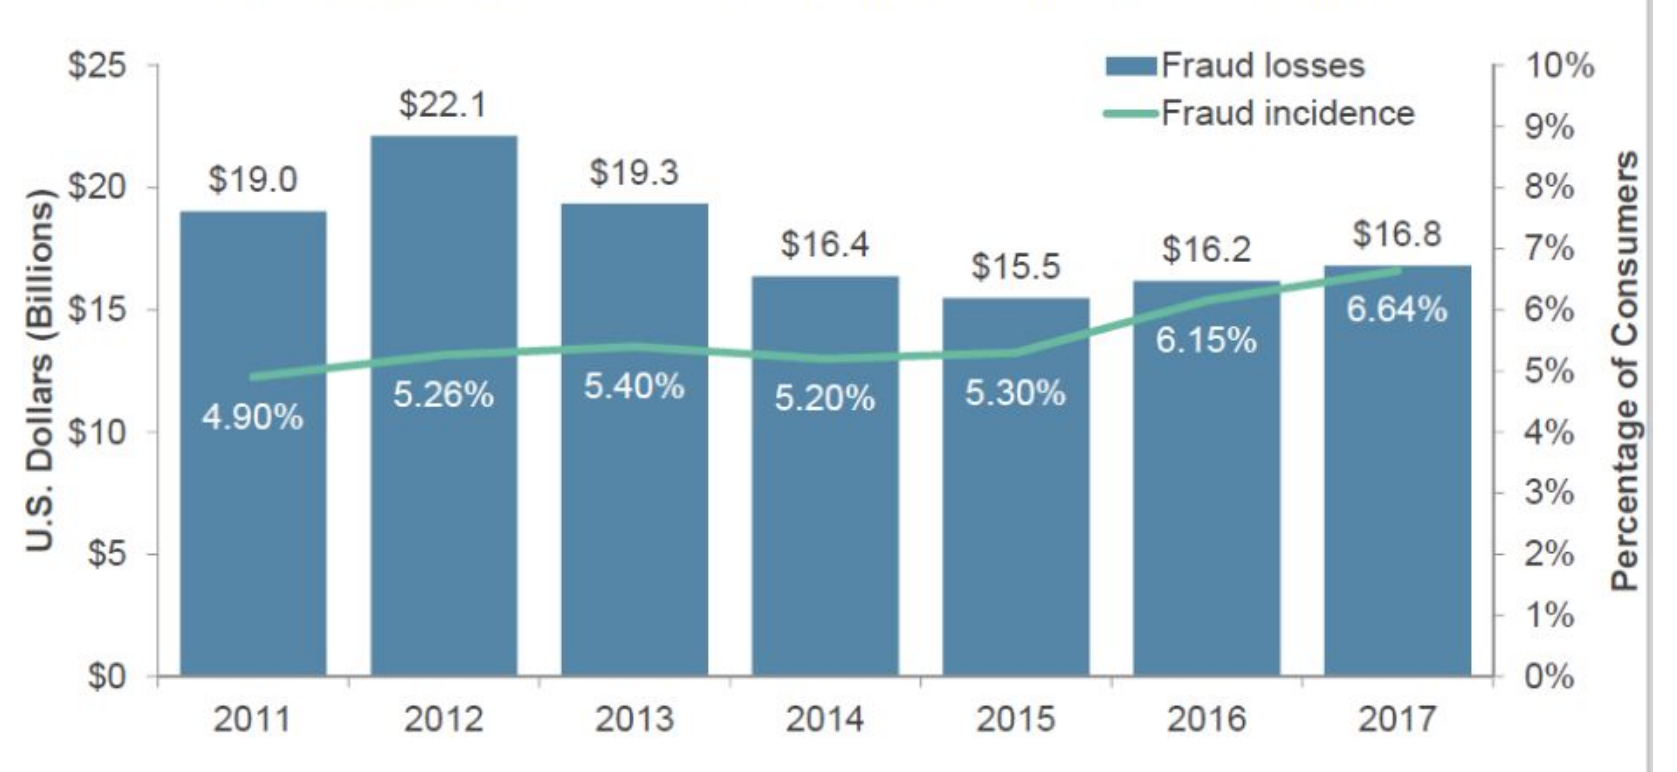
\includegraphics[scale=0.3]{11.png}
	
	
	\textit{Hình 1.1:} Tỉ lệ lừa đảo và số lượng tiền đã mất do gian giận thẻ tí dụng, 2011-2017 \footnote{Javelin Strategy \& Research 2018}
\end{center}


Một số hình thức gian lận thẻ tín dụng:
\begin{itemize}
	\item Bị thanh toán hay quẹt thẻ tại một cửa hàng nào đó khi mua hàng trong trường hợp bạn bị trộm thẻ.
	\item Sử dụng công nghệ cao qua mạng Internet đánh cắp thông tin thẻ tín dụng của người dùng.
	\item Bị rút tiền mặt qua máy ATM.
	\item Làm giả thẻ Visa, MasterCard.
	\item ...
\end{itemize}

\section{Bài toán}
Bài toán "phát hiện gian lận thẻ tín dụng" đã thu hút rất nhiều sự quan tâm nghiên cứu, một kỹ thuật đặc biệt mà một số nghiên cứu sử dụng là chú trọng vào khai thác dữ liệu và mạng neural. Trên thực tế, đã có một số cách tiếp cận để xử lý bài toán trên dựa trên tiêu chuẩn của dữ liệu trong các giao dịch chính hãng, so sánh chúng trong các trường hợp giao dịch gian lận, từ đó để phân loại các kiểu gian lận, làm tiêu chuẩn để phát hiện gian lận. Nhưng việc lấy dữ liệu các giao dịch gian lận trong thực tế là một trong những vấn đề khó khăn. Ngoài ra những phương pháp đó không thể phát hiện được các kiểu gian lận mới mà dữ liệu được dán nhãn không có sẵn. Trong bài báo cáo này, nhóm trình bày phương pháp phát hiện gian lận thẻ tín dụng dựa trên mô hình Markov ẩn (HMM). Nhóm mô hình hóa thông tin giao dịch thẻ tín dụng theo mô hình Markov ẩn. Các giao dịch chỉ có thể được quan sát thông qua quy trình ngẫu nhiên tạo ra chuỗi bao gồm số tiền thanh toán, loại hàng hóa thanh toán,... trong mỗi giao dịch. Do đó, HMM là một lựa chọn lý tưởng để giải quyết bài toán này.







\newpage
\setcounter{chapter}{1}
\chapter{Phương pháp}
\section{Mô hình Markov ẩn - Hidden Markov Model}
\subsection{Giới thiệu về mô hình Markov ẩn - Hidden Markov Model}
Mô hình Markov ẩn (HMM) được xây dựng từ những năm 1960, đây là một mô hình toán học về thống kê. Sau đó được nghiên cứu và ứng dụng rộng rãi trong nhiều lĩnh vực như: nhận dạng tiếng nói, nhận biết kí tự quang học, tin sinh học, ...

Mô hình Markov ẩn (HMM) bao gồm các thành phần:
\begin{itemize}
	\item Tập $N$ các trạng thái ẩn $S=\{S_1,\;S_2,\;S_3,\;..., \;S_N\}$ trong đó $S_i \; (i=1, 2, ...)$ là các trạng thái độc lập và không được quan sát trực tiếp từ mô hình. Ta kí hiệu trạng thái tại thời điểm $t$ là $q_t$
	\item Ma trận xác suất chuyển trạng thái $A = [a_{ij}]$ trong đó:
	$$a_{ij}=P(q_{t+1}=S_j|q_t=S_i)\text{ với }1 \leq i,\; j \leq N \quad t=1,\;2,\;...$$
	Tính chất:
	$$a_{ij} \geq 0 \quad \forall \; 1 \leq i, j \leq N \text{ và }\sum_{j=1}^{N} a_{ij}=1 \quad \forall \; 1\leq i\leq N$$
	\newpage
	\item Vector phân phối ban đầu $\pi = [\pi_i]$ trong đó:
	$$\pi_i = P(q_1=S_i) \quad \forall \; 1 \leq i \leq N $$
	Tính chất: $$\sum_{i=1}^{N}\pi_i=1$$
	\item Tập $V={V_1,\;V_2,\; ...,\; V_M}$ là tập chứa $M$ các kí hiệu quan sát khác nhau trên mỗi trạng thái.
	\item Ma trận xác suất phân bố kí hiệu quan sát trên mỗi trạng thái là $B=[b_j(k)]$ trong đó:
	$$b_j(k) = P(V_k \text{ tại thời điểm } t|q_t=S_j) \text{ với } 1\leq j \leq N, \; 1 \leq k \leq M$$
\end{itemize}

Ta kí hiệu $O=(O_1,\; O_2,\; ...,\; O_T)$ là dãy quan sát trong đó mỗi quan sát $O_i \in V$ và $T$ là số lượng các quan sát trong dãy.

Một HMM có hai đặc điểm sau:
\begin{itemize}
	\item Dãy $\{q_i\}_{i=1,\;2,\;...}$ là xích Markov trong không gian các trạng thái $S$ với ma trận xác suất chuyển trạng thái $A$ và phân phối ban đầu $\pi$.
	\item Xác suất quan sát $O_i$ xảy ra chỉ phụ thuộc vào trạng thái tạo ra quan sát $q_i$ và không phụ thuộc và bất kỳ trạng thái hay quan sát khác. Tức là:
	$$P(O_i|q_1,\; q_2,\ ...,\  q_i,\  ...,\  q_T,\  O_1,\  O_2,\  ...,\  O_{i-1},\ O_{i+1},\  ...,\  O_T) = P(O_i|q_i)$$
\end{itemize}

Tóm lại, HMM có các $O_1, O_2, \; ..., \; O_T$ được quan sát trực tiếp trong khi có một xích Markov $q_1,\; q_2,\; ..., \; q_T$ bên dưới không thể quan sát trực tiếp. Ta kí hiệu $\lambda = (A,\; B,\; \pi)$ chỉ tập tất cả các tham số trong HMM. 
\newpage
Bảng sau liệt kê các kí hiệu được sử dụng trong bài báo cáo.


\begin{tabular}{|c|l|}
	\hline 
	\textbf{Kí Hiệu} & \hspace{3.3cm} \textbf{Ý nghĩa} \\ 
	\hline 
	$N$ & Số lượng các trạng thái ẩn trong mô hình. \\ 
	\hline 
	$M$ & Số lượng các kí hiệu quan sát. \\ 
	\hline 
	$V={V_1,\;V_2,\; ...,\; V_M}$ & Tập các kí hiệu quan sát. \\ 
	\hline 
	$S=\{S_1,\;S_2,\;S_3,\;..., \;S_N\}$ & Tập các trạng thái. \\ 
	\hline 
	$A$ & Ma trận xác suất chuyển. \\ 
	\hline 
	$B$ & Ma trận phân bố quan sát trên mỗi trạng thái. \\ 
	\hline 
	$\pi$ & Vector phân phối ban đầu. \\ 
	\hline 
	$q_i$ & Trạng thái tại thời điểm thứ $i \; (i=1,\;2,\; ...,\; T)$ \\ 
	\hline 
	$O_i$ & Các quan sát tại thời điểm $i$. \\
	\hline
	$O=(O_1,\; O_2,\; ...,\; O_T)$ & Dãy các quan sát.\\
	\hline
	$\lambda = (A,\; B,\; \pi)$ & Tập toàn bộ tham số của mô hình. \\
	\hline
\end{tabular}

%\paragraph{Ví dụ:}

\subsection{Ba vấn đề cơ bản trong mô hình Markov ẩn}
Để áp dụng mô hình Markov ẩn vào các ứng dụng thực tế, trước hết ta cần có những lời giải thỏa đáng cho ba vấn đề cơ bản sau.
\begin{itemize}
	\item \textbf{Vấn đề 1 (Ước lượng):}
	Cho dãy quan sát $O=(O_1,\; O_2,\; ...,\; O_T)$ và mô hình $\lambda = (A,\; B,\; \pi)$. Xác định $P(O|\lambda)$ của dãy quan sát $O$ của mô hình đó.
	
	\item \textbf{Vấn đề 2 (Giải mã):}
	Cho dãy quan sát $O=(O_1,\; O_2,\; ...,\; O_T)$ và mô hình $\lambda = (A,\; B,\; \pi)$. Xác định dãy chuyển trạng thái $Q=Q(q_1,\; q_2,\; ...,\; q_T)$ là "tối ưu nhất" để phù hợp với dãy quan sát $O$.
	
	\item \textbf{Vấn đề 3 (Huấn luyện):}
	Điều chỉnh các tham số $\lambda = (A,\; B,\; \pi)$ để cực đại hóa $P(O|\lambda)$.
\end{itemize}

\subsubsection{Vấn đề 1 (Ước lượng - Likelihood)}
Mục tiêu của vấn đề này là tính $P(O|\lambda)$ - xác suất xảy ra $O$ từ mô hình $\lambda$. Một giải pháp đơn giản và tự nhiên là duyệt tất cả các chuỗi trạng thái $Q$ sinh ra $O$. Khi đó áp dụng công thức xác suất đầy đủ ta có:

\begin{tabular}{lll}
	$P(O|\lambda)$ & = & $\sum_{Q}P(O|Q,\; \lambda)P(Q| \lambda)$ \\ 
	& = & $\sum_{q_1,\; q_2,\; ...,\; q_T}\pi_{q_1}b_{q_1}(O_1)a_{q_1q_2}b_{q_2}(O_2)\; ... \; a_{q_{T-1}q_T}b_{q_T}(O_T)$ \\ 
\end{tabular} 

Để tìm $P(O|\lambda)$ theo cách tính trên ta cần đến $2T\times N^T$ phép tính. Điều này không khả thi ngay cả khi $N$, $T$ nhận các giá trị nhỏ. Vì vậy ta không thể tính $P(O|\lambda)$ theo cách như trên. Một giải pháp khả thi hơn để tính $P(O|\lambda)$ là sử dụng thuật toán \textit{forward} và \textit{backward}.

Đầu tiên, ta cần định nghĩa biến \textit{forward} $\alpha_t(i)$ như sau:
$$\alpha_t(i) = P(O_1,\; O_2,\; ..., \; O_t, \; q_t = S_i|\lambda)$$
là xác suất trạng thái $S_i$ ở thời điểm $t$ và các quan sát $O=(O_1,\; O_2,\; ...,\; O_t)$ từ mô hình $\lambda$.

Ta có thể tìm $P(O|\lambda)$ theo các bước sau:
\begin{itemize}
	\item Bước 1 - Khởi tạo: Đặt $\alpha_1(i) = \pi_1 b_i(O_1) \qquad 1 \leq i \leq N$
	\item Bước 2 - Quy nạp: $\forall \; t=1,\; 2,\; ...,\; T-1 \text{ và } j=1,\; 2,\; ...,\;N$
	$$\alpha_{t+1} = b_j(O_{t+1})\sum_{j=1}^{N} \alpha_t(j)a_{ij}$$
	\item Bước 3 - Kết thúc: Tính $$P(O|\lambda)=\sum_{i=1}^{N}\alpha_T(i)$$
\end{itemize}

Thuật toán trên được gọi là thuật toán \textit{forward}. Thuật toán yêu cầu $T\times N^2$ phép tính, nhỏ hơn rất nhiều so với phương pháp tính trực tiếp ở trên.

Tương tự như thuật toán \textit{forward}, ta có thể giải quyết vấn đề bằng thuật toán \textit{backward}. Trước hết, ta định nghĩa biến \textit{backward} như sau:
$$\beta_t(i)=P(O_{t+1},\; O_{t+2},\; ...,\; O_T|q_t=S_i,\lambda)$$
là xác suất quan sát được dãy $O=(O_1,\; O_2,\; ...,\; O_T)$ biết mô hình $\lambda$, $S_i$ là trạng thái tại thời điểm thứ t.

Thuật toán \textit{backward} thực hiện như sau:
\begin{itemize}
	\item Bước 1 - Khởi tạo: Đặt $\beta_T(i) = 1 \qquad 1 \leq i \leq N$
	\item Bước 2 - Quy nạp: $\forall \; t=T-1,\; T-2,\; ...,\; 1 \text{ và } i=1,\; 2,\; ...,\;N$
	$$\beta_t = \sum_{j=1}^{N} a_{ij}b_j (O_{t+1})\beta_{t+1}(j)$$
	\item Bước 3 - Kết thúc: Tính $$P(O|\lambda)=\sum_{j=1}^{N}\pi_j b_j(O_1)\beta_1(j)$$
\end{itemize}

Cũng giống như thuật toán \textit{forward}, thuật toán \textit{backward} yêu cầu $T\times N^2$ phép tính. Vì vậy cả hai thuật toán \textit{forward} và \textit{backward} đều khả thi với chi phí hoàn toàn chấp nhận được\footnote{Chi tiết chứng minh về thuật toán xem tại tài liệu [1]}

\subsubsection{Vấn đề 2 (Giải mã - Decoding)}
Mục tiêu của vấn đề 2 là tìm ra chuỗi trạng thái "tối ưu" nhất $Q=\{q_1,\;q_2,\;...,\;q_T\}$ đã phát sinh ra $O$. Một điều đáng lưu ý là có rất nhiều các tiêu chí "tối ưu" được chọn. Một trong những tiêu chí đó là chọn ra từng $q_t$ có độ khả thi cao nhất ở từng thời điểm $t$ thông qua độ đo xác suất $P(q_t=S_i|O,\; \lambda)$ - xác suất ở trạng thái $S_i$ vào thời điểm t cho trước $t$ cho trước chuỗi tín hiệu quan sát $O$ và mô hình $\lambda$. Ta gọi độ đo này $\gamma_t(i)$:
$$\gamma_t(i)=P(q_t=S_i|O,\; \lambda)$$ 
Biến $\gamma_t(i)$ có thể được tính thông qua các biết $\alpha_t(i)$ và $\beta_t(i)$ theo biểu thức:
$$\gamma_t(i) = \frac{\alpha_t(i)\beta_t(i)}{P(O|\lambda)}=\frac{\alpha_t(i)\beta_t(i)}{\sum_{i=1}^{N}\alpha_t(i)\beta_t(i)}$$
Thông qua biến $\gamma_t(i)$, ta hoàn toàn có thể xác định được trạng thái có khả năng cao nhất đạt đến ở thời điểm $t$:
$$q_t=arg
\max_{1\leq i\leq N}[\gamma_t(i)], \qquad 1 \leq t \leq T$$

Tuy nhiên, kết quả này chỉ mang tính cục bộ, nghĩa là đôi khi chuỗi $Q$ tìm được không tồn tại trong thực tế nếu một số xác suất chuyển trạng thái bằng 0. 

Để tránh tình trạng mâu thuẫn như trên, ta có thể thay đổi tiêu chí "tối ưu" cho việc chọn $Q$. Tùy theo từng ứng dụng cụ thể mà tiêu chí này sẽ được chọn sao cho phù hợp, tuy nhiên tiêu chí phổ biến nhất được sử dụng là chọn cả chuỗi $Q$ khả thi nhất, nghĩa là qui bài toán từ việc tìm Q để cực đại hóa $P(Q|O,\;\lambda)$. Giải pháp cho vấn đề này là thuật toán Viterbi.

Thuật toán Viterbi định nghĩa biến $\delta_t(i)$ là xác suất cao nhất của đoạn chuỗi trạng thái dẫn đến trạng thái $S_i$ ở thời điểm $t$ và đã quan sát được đoạn $O_1,\; O_2,\; ...,\; O_t$ cho trước mô hình $\lambda$:
$$\delta_t(i) = \max_{q_1, \; q_2,\; ...,\; q_t} P(q_1, \; q_2,\; ...,\; q_t=S_i,\; O_1O_2\; ...\;O_t|\lambda)$$

Biến $\delta_t(i)$ được tính theo quy nạp với các bước sau đây (thuật toán Viterbi):
\begin{itemize}
	\item Bước 1 - Khởi tạo:
	$$\delta_t(i)=\pi_i b_i(O_1), \qquad 1\leq i \leq N$$
	\item Bước 2 - Lặp quy nạp:
	$$\delta_t(j)=\max_{1\leq i\leq N}[\delta_{t-1}(i)a_{ij}]b_j(O_t), \qquad 2\leq t \leq T,\; 1 \leq j \leq N $$
	$$\psi(j)=\max{1\leq i \leq N}[\delta_{t-1}(i)a_{ij}], \qquad 2\leq t \leq T,\; 1 \leq j \leq N$$
	\item Bước 3 - Kết thúc lặp:
	$$p^{*}=\max{1\leq i \leq N}[\delta_T(i)]$$
	$$q_t^{*}=arg \max{1\leq i \leq N}[\delta_T(i)]$$
	\item Bước 4 - Quay lui:
	$$q_t^{*}=\psi_{t+1}(q_{t+1}^{*}), \qquad t=T-1,\; T-2,\; ...,\; 1$$
\end{itemize}
Kết thúc thuật toán, chuỗi $Q=q_1^{*}q_2^{*}\; ... q_T^{*}$ chính là lời giải đáp thỏa đáng của vấn đề trên.\footnote{Chi tiết chứng minh về thuật toán xem tại tài liệu [1]}


\subsubsection{Vấn đề 3 (Huấn luyện - Learning)}
Mục tiêu của vấn đề thứ ba - cũng là vấn đề phức tạp nhất là tìm cách điều chỉnh các tham số của mô hình $\lambda=(A,B,\pi)$ để cực đại hóa $P(O|\lambda)$. Với dãy quan sát $O$ là dữ liệu huấn luyện, bộ tham số $\lambda$ của mô hình có thể xác định sao cho $P(O|\lambda)$ đạt cực đại tại địa phương bằng thuật toán Baum - Welch. Trước tiên ta định nghĩa $\xi_t(i,\; j)$ như sau:
$$\xi_t(i,\; j)=P(q_t=S_i,\; q_{t+1}=S_j|O,\; \lambda)$$
là xác suất trạng thái $S_i$ ở thời điểm $t$ và $S_j$ ở thời điểm $t+1$ khi biết mô hình $\lambda$ và dãy các quan sát $O$. Ta có thể tính $\xi_t(i,\; j)$ thông qua các biến $\alpha_t(i)$ và $\beta_t(i)$:
\begin{center}
	\begin{tabular}{lll}
		$\xi_t(i,\; j)$ & = & $\frac{\alpha_t(i)a_{ij}b_j(O_{t+1})\beta_{t+1}(j)}{P(O|\lambda)}$ \\ 
		& = & $\frac{\alpha_t(i)a_{ij}b_j(O_{t+1})\beta_{t+1}(j)}{\sum_{i=1}^{N}\sum_{j=1}^{N}\alpha_t(i)a_{ij}b_j(O_{t+1})\beta_{t+1}(j)}$ \\ 
	\end{tabular}
\end{center}
Chúng ta đã định nghĩa ở phần trước $\gamma_t(i)$ (trong phần thuật toán Viterbi) là xác suất trạng thái $S_i$ ở thời gian t khi biết mô hình $\lambda$ và dãy quan sát. Do đó, ta có mối quan hệ sau:
$$\gamma_t(i)=\sum_{j=1}^{N}\xi_t(i,\;j)$$
Hơn nữa, ta có:
$$\sum_{t=1}^{T-1}\gamma_t(i)=\text{trung bình số lần chuyển trạng thái từ } S_i$$
$$\sum_{t=1}^{T-1}\xi_t(i,\;j)=\text{trung bình số lần chuyển trạng thái từ } S_i \text{ sang } S_j$$
\newpage
Từ những điều trên ta rút ra các bước của thuật toán Baum - Welch giải quyết vấn đề:
\begin{itemize}
	\item Bước 1: Khởi tạo ngẫu nhiên các tham số $\lambda = (A,B,\pi)$.
	\item Bước 2: Tính toán $\alpha_t(i),\; \beta_t(i),\; \xi_t(i,\;j),\gamma_t(i) \text{ với } t = 1,\; 2,\; ...,\; T, \; 1 \leq i,\; j \leq N$.
	\item Bước 3: Cập nhật các tham số $\overline{\lambda} = (\overline{A},\; \overline{B},\; \overline{\pi})$:
	$$\overline{\pi_i} = \gamma_1(i)$$
	$$\overline{a}_{ij} = \frac{\sum_{t=1}^{T-1}\xi_t(i,\;j)}{\sum_{t=1}^{T-1}\gamma_t(i)}$$
	$$\overline{b}_{ij}(k) = \frac{\sum_{t=1,\; O_t=V_k}^{T}\gamma_t(i)}{\sum_{t=1}^{T}\gamma_t(i)}$$
	\item Bước 4: Nếu $P(O|\overline{\lambda})$ tăng quay lại bước 2, ngược lại thì dừng thuật toán.
\end{itemize}
Từ đó ta rút ra được $\overline{\lambda} = (\overline{A},\; \overline{B},\; \overline{\pi})$ là các tham số mới của mô hình. Theo Baum đã chứng minh, ta luôn có $P(O,\; \overline{\lambda}) > P(O|\lambda)$ cho đến khi mô hình đã đạt đến cực đại địa phương \footnote{Chi tết thêm về thuật toán và các chứng minh xem trong tài liệu [1], [4]}.

\section{Áp dụng HMM vào bài toán phát hiện gian lận thẻ tín dụng}
Sau đây, nhóm sẽ áp dụng mô hình Markov ẩn để xây dựng một hệ thống phát hiện gian lận thẻ tín dụng. Hệ thống được sử dụng trong các ngân hàng - nơi phát hành thẻ tín dụng và quản lý các giao dịch. Hệ thống sẽ nhận các thông tin chi tiết về thẻ và số tiền mua hàng trong mỗi giao dịch để dự đoán giao dịch đó có phải gian lận không. Các loại hàng hóa được mua trong mỗi giao dịch không được biết đến. Nếu hệ thống phát hiện các giao dịch đó là gian lận, ngân hàng sẽ tạm dừng giao dịch và gửi cảnh báo đến chủ thẻ để xác minh giao dịch. 
%\subsection{Mô hình hóa và tiền xử lý dữ liệu}
\subsection{Mô hình hóa}
Chúng ta  xây dựng đối với mỗi chủ thẻ là một mô hình Markov ẩn và dựa vào lịch sử giao dịch của chủ thẻ để phát hiện ra các giao dịch gian lận. Trước tiên, ta cần chỉ rõ các kí hiệu quan sát (\textit{observation symbols}) trong mô hình. Ta sẽ chia các giao dịch thành ba phần dựa trên các thuộc tính của giao dịch như là số tiền giao dịch, ngày thực hiện giao dịch (có phải cuối tuần hay ngày lễ không?),... Tuy nhiên do hạn chế về dữ liệu có được nên ta sẽ chia các giao dịch của chủ thẻ dựa vào số tiền giao dịch thành ba nhóm: số tiền giao dịch thấp ($l$), số tiền giao dịch trung bình ($m$), số tiền giao dịch cao ($h$). Ba nhóm có thể được xác định dễ dàng bằng \textit{thuật toán phân cụm} trên các giao dịch của chủ thẻ. Chúng ta chọn $V = \{l, m, h\}$ là tập hợp các kí hiệu quan sát của mô hình. Ví dụ: Với chủ thẻ A, dựa vào lịch sử giao dịch, ta xác định được $l = (0,\; 200 \$ ], \; m = (200 \$ ,\; 400 \$ ),\; h = [400 \$ ,\text{ giới hạn của thẻ tín dụng}]$. Nếu chủ thẻ A thực hiện một giao dịch với số tiền giao dịch là $100 \$ $ thì mô hình nhận được quan sát là $l$. 


Tiếp theo ta cần chỉ rõ tập các trạng thái ẩn của mô hình. Ta thấy trong mỗi giao dịch, chủ thẻ mua các mặt hàng khác nhau với số tiền khác nhau. Một chủ thẻ thực hiện giao dịch phụ thuộc vào nhu cầu mua sắm các mặt hàng khác nhau của người đó. Ta thấy rằng số tiền giao dịch thường phụ thuộc vào mặt hàng mà người đó mua. Mặt khác, ngân hàng thường không biết được chi tiết các mặt hàng mà chủ thẻ mua trong giao dịch. Do đó, ta có thể mô hình hóa loại mặt hàng như là trạng thái ẩn trong mô hình. Ví dụ: Tập các trạng thái ẩn như: {đồ điện tử, đồ chơi trẻ em, thực phẩm, ...}. Ta thấy chủ thẻ có thể mua nhiều loại mặt hàng khác nhau trong một giao dịch. Tuy nhiên, chúng ta không cố gắng xác định các loại mặt hàng nào đã được mua trong mỗi giao dịch. Vì các thông tin đó mang tính dự đoán trong ngân hàng nên đối với hệ thống phát hiện gian lận chúng thường không có giá trị.

Vậy chúng ta mô hình hóa loại mặt hàng là trạng thái ẩn và số tiền mua trong mỗi giao dịch là một quan sát trong mô hình Markov ẩn.

\subsection{Tiền xử lý dữ liệu}
Như đã trình bày ở trên, đối với mỗi chủ thẻ, chúng ta xây dựng và huấn luyện một mô hình Markov ẩn. Để xác định các quan sát tương ứng với mỗi giao dịch của chủ thẻ, chúng ta sử dụng thuật toán phân cụm trên các giao dịch trong lịch sử của chủ thẻ. Thông thường, các giao dịch được lưu trữ trong cơ sở dữ liệu của ngân hàng chứa nhiều các thuộc tính. Tuy nhiên do dữ liệu còn hạn chế, ta chỉ xem xét số tiền mà chủ thẻ đã sử dụng trong mỗi giao dịch. Ta sử dụng thuật toán phân cụm K-means để xác định các cụm. K-means là một thuật toán máy học không giám sát. Mục đích là chia dữ liệu thành các cụm khác nhau sao cho dữ liệu trong cùng một cụm có các tính chất giống nhau. Số lượng cụm K được cố định ngay từ đầu. Việc phân cụm được thực hiện bằng cách cực tiểu hóa tổng bình phương khoảng cách giữa các điểm dữ liệu với tâm cụm.

Như đề cập ở phía trên, số lượng các kí hiệu quan sát là ba: $(l,\; m,\; h)$, do đó số lượng cụm K = 3. Giả sử $c_l,\; c_m,\; c_h$ là tâm của 3 cụm hay giá trị trung bình được tạo tương ứng với  $l,\; m,\; h$. Các điểm này được dùng để xác định các quan sát khi có giao dịch mới. Giả sử $x$ là số tiền giao dịch của chủ thẻ $A$ trong giao dịch thứ $T$. Khi đó, hệ thống xác định được quan sát tương ứng cho $x$ (kí hiệu là $Ox$) là: 
$$O_x=V_{\argmin_i(|x-c_i|)}$$

Nói cách khác, hệ thống sẽ xác định quan sát cho mỗi giao dịch ứng với cụm mà có khoảng cách nhỏ nhất từ giá tiền đến tâm cụm. \footnote{chi tiết về thuật toán K-means xem trong tài liệu [6]}

\subsection{Huấn luyện}
Sau khi mô hình hóa, chúng ta sử dụng thuật toán Baum – Welch để đào tạo xác định các tham số $(A,\; B,\; \pi)$ của mô hình. Như đã trình bày trong phần 2.1.2, thuật toán ban đầu sẽ khởi tạo các tham số $(A,\; B,\; \pi)$. Việc khởi tạo giá trị của các tham số này ảnh hưởng đến tốc độ hội tụ và nghiệm tối ưu của bài toán. Ở đây, ta sẽ khởi tạo phân phối ban đầu $\pi$ là phân phối đều. Ví dụ: có $N$ trạng thái ẩn thì xác suất ban đầu của mỗi trạng thái là $\frac{1}{N}$. Khởi tạo ma trận xác suất chuyển $A$ và ma trận phân bố quan sát $B$ cũng có thể coi là đều. Tuy nhiên, để khởi  tạo ma trận B chính xác hơn, ta có thể sử dụng phương pháp thống kê khảo sát với nhiều người để ước lượng được xác suất mua loại mặt hàng nào đó với số tiền thuộc nhóm thấp, trung bình, cao. Trong khi đó, ma trận A sẽ được khởi tạo theo phân phối đều.
Sau khi khởi tạo, chúng ta bắt đầu huấn luyện các tham số của mô hình sao cho xác suất xảy ra dãy các quan sát từ lịch sử giao dịch của chủ thẻ là lớn nhất. Kết thúc quá trình huấn luyện ta sẽ nhận được bộ các tham số $(A,\; B,\; \pi)$ của mô hình Markov ẩn ứng với mỗi chủ thẻ. Kết thúc quá trình huấn luyên chúng ta chuyển sang quá trình dự đoán, phát hiện gian lận.

\subsection{Phát hiện gian lận}
Sau khi huấn luyện các tham số của mô hình HMM, chúng ta lấy các quan sát từ dữ liệu đào tạo của chủ thẻ tạo thành một dãy các quan sát cơ sở. Giả sử dãy quan sát ban đầu là $(O_1,\; O_2,\; ...,\; O_R)$ là lịch sử $R$ giao dịch của chủ thẻ đến thời điểm t. Ta tính xác suất để quan sát được dãy trên:
$$\theta_1=P(O_1,\; O_2,\; ...,\; O_R|\lambda)$$
Giả sử $O_{R+1}$ là quan sát xuất hiện trong giao dịch mới của chủ thẻ tại thời điểm $t+1$. Khi đó, ta sẽ có dãy $(O_2,\; O_3,\; ...,\; O_R,\; O_{R+1})$ là dãy mới. Ta cũng tính xác suất quan sát được dãy trên:
$$\theta_2=P(O_2,\; O_3,\; ...,\; O_{R+1}|\lambda)$$

Khi đó, đặt: $\Delta \theta = \theta_1 - \theta_2$. Nếu $\Delta \theta > 0$ tức là xác suất xuất hiện dãy mới thấp hơn dãy cũ thì nó có thể là một gian lận. Các giao dịch mới được dự đoán là gian lận nếu:
$$\frac{\Delta \theta}{\theta_1} \geq \epsilon$$
Giá trị $\epsilon$ được gọi là giá trị ngưỡng. Nếu $O_{R+1}$ được xác định là gian lận khi đó hệ thống sẽ loại bỏ quan sát trên và vẫn sử dụng dãy $(O_1,\; O_2,\; ...,\; O_R)$ là dãy cơ sở. Ngược lại, hệ thống sẽ chọn dãy $(O_2,\; O_3,\; ...,\; O_{R+1})$ là dãy cơ sở cho lần dự đoán tiếp theo. Ý tưởng của phương pháp này dựa trên thói quen chi tiêu của chủ thẻ. Khi có một hành vi chi tiêu bất thường thì nhiều khả năng sẽ là gian lận. Khi đó ngân hàng sẽ tạm dừng giao dịch, và gửi cảnh báo đến chủ thẻ để yêu cầu xác minh giao dịch.


\newpage
\setcounter{chapter}{2}
\chapter{Kết quả}
\section{Mô tả dữ liệu}
Dữ liệu nhóm thu thập được bao gồm 4 file csv sau:
\begin{itemize}
	\item File CustomberBase.csv chứa thông tin của 5674 khác hàng với các thuộc tính như Cust\_ID - mã số của khách hàng, Age - là tuổi của khách hàng, Customer\_Segment - hạng của khách hàng, Customer\_Vintage\_Group - nhóm khách hàng thuộc vào.
	\item File CardBase.csv chứa thông tin của 500 thẻ tương ứng với 500 chủ sở hữu trong 5674 người thuộc file CustomberBase.csv. File này chứa các thuộc tính Card\_Number - số thẻ, Card\_Family - loại thẻ, Credit\_Limit - số tiền giới hạn của thẻ, Cust\_ID - mã số của chủ thẻ.
	\item File TransactionBase.csv chứa thông tin của các giao dịch trong năm 2016 tương ứng với thẻ trong file CardBase.csv. File này chứa các thuộc tính Transaction\_ID - mã số giao dịch, Transaction\_Date - thời gian giao dịch, Credit\_Card\_ID - số thẻ tham gia giao dịch, Transaction\_Value - số lượng tiền giao dịch, Transaction\_Segment - phân lớp giao dịch.
\end{itemize}
\textit{Chú ý:} Lý do bảo mật nên mọi thông tin về số thẻ, khách hàng, lượng tiền giao dịch đều đã bị thay đổi.

Ta biến đổi dữ liệu trên thành các file csv, mỗi file chứa thông tin giao dịch của chủ thẻ trong năm 2016, được chia thành hai phần: dữ liệu giao dịch đầu tiên tới giao dịch áp chót dùng trong việc luyện mô hình, giao dịch cuối cùng cho việc kiểm tra mô hình. Tổng số dữ liệu kiểm tra là 470 giao dịch trong đó gồm: 67 giao dịch có nhãn gian lận và 403 giao dịch chính thống.

Dữ liệu giao dịch của mỗi người rất ít, mỗi thẻ chỉ có 6 - 20 giao dịch cho việc luyện mô hình. Đây là hạn chế lớn của dữ liệu, ảnh hưởng không tốt tới kết quả của mô hình.

Từ những dữ liệu nhóm đã có sẵn, với mỗi chủ thẻ, ta xây dựng mô hình Markov ẩn với số lượng lớp ẩn là 4, số lượng kí hiệu quan sát là 3, các ma trận $A,\; B,\; \pi$ đều được khởi tạo với phân phối đều.

\section{Kết quả}
Các tiêu chuẩn để đánh giá mô hình:
\begin{itemize}
	\item Accuracy - tỷ lệ số lượng dự đoán đúng so với số lượng dữ liệu kiểm tra.
	\item Confusion matrix 
	
	$$
	\begin{bmatrix} 
		TN & FP \\
		FN & TP \\
	\end{bmatrix}
	$$

	TP (True positive) - số lượng giao dịch gian lận được dự đoán chính xác.
	
	FP (False positive) - số lượng giao dịch chính thống nhưng bị dự đoán là gian lận.
	
	TN (True negative) - số lượng giao dịch chính thống được dự đoán chính xác.
	
	FP (False Negative) - số lượng giao dịch gian lận nhưng bị dự đoán là chính thống.
	\item Precision: $$\frac{TP}{TP+FP}$$
	\item Recall:
	$$\frac{TP}{TP+FN}$$
\end{itemize}

Với ngưỡng là $0.4$ ta thu được các kết quả đánh giá sau:
\begin{itemize}
	\item Accuracy$=0.9$.
	\item Precision$=0.622$.
	\item Recall$=0.7612$.
	\item Confusion matrix:
	
	$$
	\begin{bmatrix} 
	372 & 31 \\
	16 & 51 \\
	\end{bmatrix}
	$$
	
\end{itemize}

Với bộ dữ liệu còn thiếu hụt thì mô hình trên ổn nhưng chưa đủ để ứng dụng vào thực tế.

Khảo sát sự thay đổi của ngưỡng ảnh hưởng tới kết quả của mô hình:
\begin{center}
	
	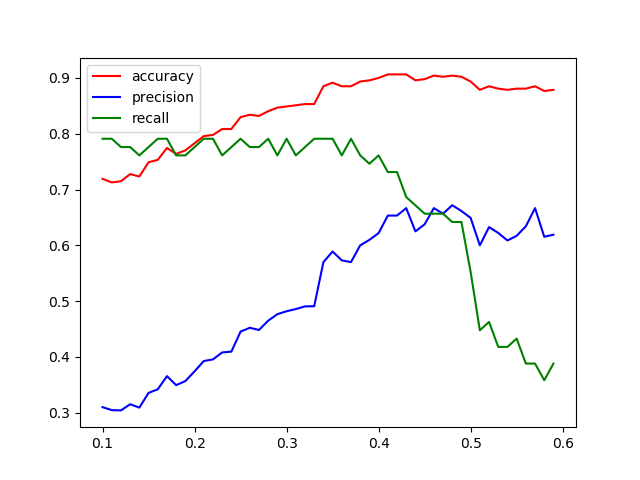
\includegraphics[scale=1]{31.png}
	
	
	\textit{Hình 3.1:} Đồ thị thể hiện sự ảnh hưởng của ngưỡng.
\end{center}
Từ hình trên ta thấy việc chọn ngưỡng rất quan trọng. Nếu ngưỡng quá cao hệ thống sẽ bỏ qua nhiều gian lận trong khi nếu ngưỡng quá thấp thì hệ sẽ báo nhiều giao dịch chính thống là gian lận.



\newpage
\input {Tongket}

\newpage
\input {Ketluan}

\newpage
\input {Tailieuthamkhao}

\end{document}